
\begin{figure}[!h]
    \centering
    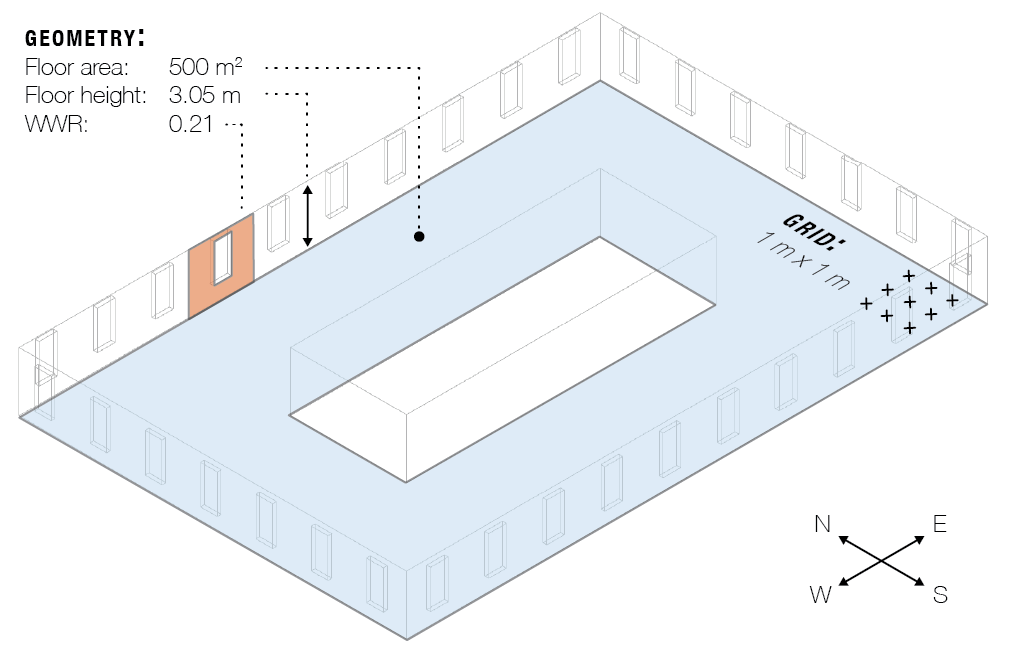
\includegraphics[width=0.8\textwidth]{manuscript/src/figures/sim-geometry.png}
    \vspace{0.5cm}
    % \caption{Geometry of case study model.}

        \renewcommand{\arraystretch}{1.5}
    

        \begin{tabular}{ p{3.5cm} p{2cm} p{2cm} p{2cm} }
        
            \hline
            
            {\textbf{Setting(s)}} & \multicolumn{3}{l}{\textbf{Definition}} \\
        
            \hline
        
            {Climates}  & \multicolumn{3}{l}{Brisbane (Cfa)} \\
        
            % \cline{2-3}
            
            {Constructions} & \multicolumn{3}{l}{\textit{ASHRAE 90.1 2019, IECC 2021}, Steel-framed*} \\
        
            % \cline{2-3}  
            
            {Program} & \multicolumn{3}{l}{\textit{Small Office*}} \\
            
            % \cline{2-3}
        
            {HVAC system} & \multicolumn{3}{l}{\textit{IdealAir system}, \textit{Air conditioned}} \\
        
            % \cline{2-3}

            {\textbf{Case}} & {a) \textbf{Baseline}} & {b) \textbf{Mixed-Mode}} & {c) \textbf{PCS}} \\

            \cline{2-4}
        
            {Strategy} & {Standard} & {Mixed-Mode} & {Mixed-Mode} \\

             % \cline{2-3}

            {\textit{Passive\newline measures}} & {-} & {NV \newline Ext. shading\newline $U_{win} = 1.3$\newline $U_{wall} = 0.2$} & {PCS\newline NV\newline Ext. shading\newline $U_{win} = 1.3$\newline $U_{wall} = 0.2$} \\

             % \cline{2-3}
        
            {Setpoint range\newline \textit{Heating - Cooling}} & {22-24\degree C} & {21-25\degree C} & {19-27\degree C} \\
            
            \hline
        
        \end{tabular}
        \vspace{0.5cm}
        \caption{Overview of main settings for simulated case study scenarios: Construction properties, loads and schedules were based on Department of Energy (DOE) reference building information. (NV - Natural ventilation, U - U value in W/m²K)}
        \label{tab:sim-settings}
        

\end{figure}